\documentclass{article}
\usepackage{tikz}

\begin{document}

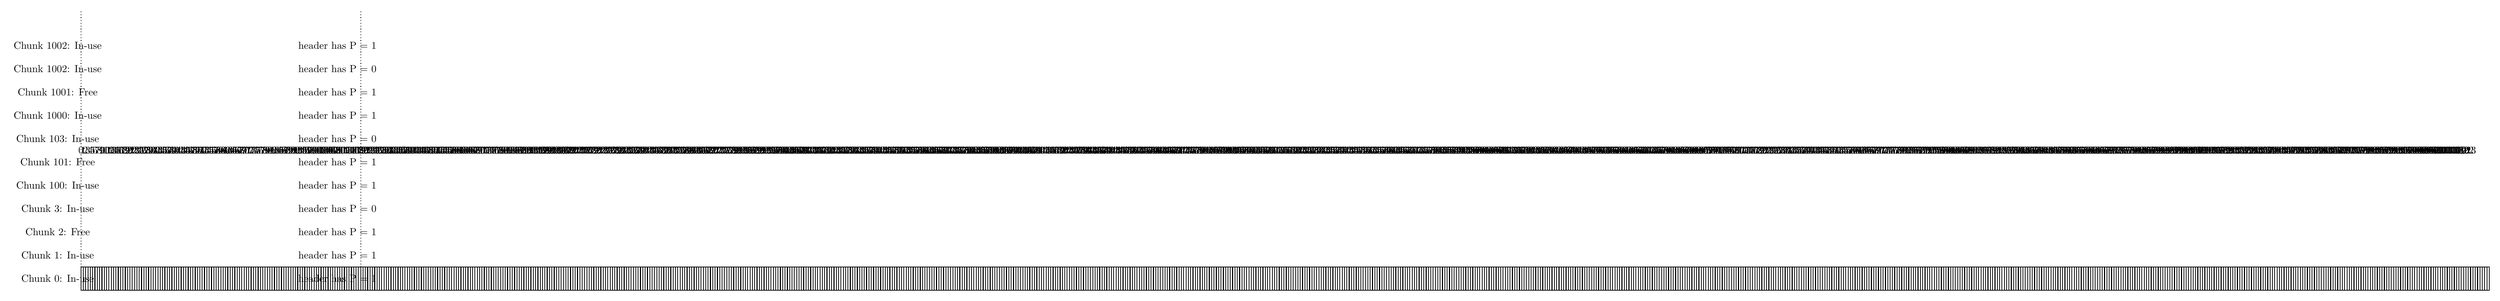
\begin{tikzpicture}[scale=0.8]
    \draw[thick,dotted] (0,0) -- (0,12);
    \draw[thick,dotted] (12,0) -- (12,12);

    \foreach \x in {0,...,1023} {
        \node at (\x/10,6) {\x};
    }

    \foreach \y [count=\i from 0] in {Chunk 0: In-use, Chunk 1: In-use, Chunk 2: Free, Chunk 3: In-use, Chunk 100: In-use, Chunk 101: Free, Chunk 103: In-use, Chunk 1000: In-use, Chunk 1001: Free, Chunk 1002: In-use, Chunk 1002: In-use} {
        \node at (-1,\i+0.5) {\y};
    }

    \foreach \y [count=\i from 0] in {header has P = 1, header has P = 1, header has P = 1, header has P = 0, header has P = 1, header has P = 1, header has P = 0, header has P = 1, header has P = 1, header has P = 0, header has P = 1} {
        \node at (11,\i+0.5) {\y};
    }

    \foreach \x in {0,...,1023} {
        \draw[thick] (\x/10,0) rectangle ++(1,1);
    }
\end{tikzpicture}

\end{document}